\synctex=1

\documentclass[10pt,notheorems]{beamer}

\usepackage{etex}
\usepackage{fourier-orns}
\usepackage{ccicons}
\usepackage{amssymb}
\usepackage{amstext}
\usepackage{amsbsy}
\usepackage{amsopn}
\usepackage{amscd}
\usepackage{amsxtra}
\usepackage{amsthm}
\usepackage{float}
\usepackage{color, colortbl}
\usepackage{mathrsfs}
\usepackage{bm}
\usepackage[nice]{nicefrac}
\usepackage{setspace}
\usepackage{ragged2e}
\usepackage{minted}
\usepackage{algorithms/algorithm}
\usepackage{algorithms/algorithmic}
\usepackage[frenchb]{babel}
\usepackage{pgf}
\usepackage{import}
\usepackage{tikz,pgfplots,pgfplotstable}
\pgfplotsset{compat=newest}
\usetikzlibrary{patterns, arrows, decorations.pathreplacing, decorations.markings, decorations.text, calc}
\pgfplotsset{plot coordinates/math parser=false}
\newlength\figureheight
\newlength\figurewidth
%\usepackage[utf8x]{inputenc}
\usepackage{cancel}
\usepackage{tikz-qtree}
\usepackage{dcolumn}
\usepackage{adjustbox}
\usepackage{environ}
\usepackage[cal=boondox]{mathalfa}
\usepackage{manfnt}
\usepackage{hyperref}
\hypersetup{
  colorlinks=true,
  linkcolor=blue,
  filecolor=black,
  urlcolor=black,
}
\usepackage{venndiagram}
\usepackage{scrextend}
\usepackage[normalem]{ulem}

% Git hash
\usepackage{xstring}
\usepackage{catchfile}
\immediate\write18{git rev-parse HEAD > git.hash}
\CatchFileDef{\HEAD}{git.hash}{\endlinechar=-1}
\newcommand{\gitrevision}{\StrLeft{\HEAD}{7}}

\newcommand{\trace}{\mathrm{tr}}
\newcommand{\vect}{\mathrm{vec}}
\newcommand{\tracarg}[1]{\mathrm{tr}\left\{#1\right\}}
\newcommand{\vectarg}[1]{\mathrm{vec}\left(#1\right)}
\newcommand{\vecth}[1]{\mathrm{vech}\left(#1\right)}
\newcommand{\iid}[2]{\mathrm{iid}\left(#1,#2\right)}
\newcommand{\normal}[2]{\mathcal N\left(#1,#2\right)}
\newcommand{\dynare}{\href{http://www.dynare.org}{\color{blue}Dynare}}
\newcommand{\sample}{\mathcal Y_T}
\newcommand{\samplet}[1]{\mathcal Y_{#1}}
\newcommand{\slidetitle}[1]{\fancyhead[L]{\textsc{#1}}}

\newcommand{\R}{{\mathbb R}}
\newcommand{\C}{{\mathbb C}}
\newcommand{\N}{{\mathbb N}}
\newcommand{\Z}{{\mathbb Z}}
\newcommand{\binomial}[2]{\begin{pmatrix} #1 \\ #2 \end{pmatrix}}
\newcommand{\bigO}[1]{\mathcal O \left(#1\right)}
\newcommand{\red}{\color{red}}
\newcommand{\blue}{\color{blue}}

\newcommand*\circled[1]{\tikz[baseline=(char.base)]{
    \node[shape=circle,draw,inner sep=1.0pt] (char) {#1};}}

\renewcommand{\qedsymbol}{C.Q.F.D.}

\newcolumntype{d}{D{.}{.}{-1}}
\definecolor{gray}{gray}{0.9}
\newcolumntype{g}{>{\columncolor{gray}}c}

\setbeamertemplate{theorems}[numbered]

\theoremstyle{plain}
\newtheorem{theorem}{Théorème}

\theoremstyle{definition} % insert bellow all blocks you want in normal text
\newtheorem{definition}{Définition}
\newtheorem{properties}{Propriétés}
\newtheorem{lemma}{Lemme}
\newtheorem{assumption}{Hypothèse}
\newtheorem{property}[properties]{Propriété}
\newtheorem{example}{Exemple}
\newtheorem*{idea}{Éléments de preuve} % no numbered block

\setbeamertemplate{footline}{
  {\hfill\vspace*{1pt}\href{http://creativecommons.org/licenses/by-sa/3.0/legalcode}{\ccbysa}\hspace{.1cm}
    \raisebox{-.1cm}{\href{https://github.com/stepan-a/growth}{\includegraphics[scale=.015]{../img/git.png}}}\enspace
    \href{https://github.com/stepan-a/growth/blob/\HEAD/cours/education.tex}{\gitrevision}\enspace--\enspace\today\enspace
  }}

\setbeamertemplate{navigation symbols}{}
\setbeamertemplate{blocks}[rounded][shadow=true]
\setbeamertemplate{caption}[numbered]


\NewEnviron{notes}{\justifying\tiny\begin{spacing}{1.0}\BODY\vfill\pagebreak\end{spacing}}

\newenvironment{exercise}[1]
{\bgroup \small\begin{block}{Ex. #1}}
  {\end{block}\egroup}

\newenvironment{defn}[1]
{\bgroup \small\begin{block}{Définition. #1}}
  {\end{block}\egroup}

\newenvironment{exemple}[1]
{\bgroup \small\begin{block}{Exemple. #1}}
  {\end{block}\egroup}


\begin{document}

\title{Croissance\\\small{Modèle de Solow avec capital humain}}
\author[S. Adjemian]{Stéphane Adjemian}
\institute{\texttt{stephane.adjemian@univ-lemans.fr}}
\date{Novembre 2022}

\begin{frame}
  \titlepage{}
\end{frame}


\begin{frame}

  \begin{itemize}

  \item Le modèle de Solow, n'est pas quantitativement satisfaisant~:
    \medskip
    \begin{itemize}
    \item Les élasticités ont les signes attendus mais les restrictions sur celles-ci sont rejetés par les données.
    \item La vitesse de convergence est bien positive, mais elle est moins importante que suggéré par le modèle.\newline
    \end{itemize}

  \item Pour rapprocher la vitesse de convergence théorique de nos mesures, il
    faudrait pouvoir accroître la valeur de $\alpha$, c'est-à-dire réduire la
    rémunération du travail dans la valeur ajoutée.\newline
    \[
      \beta = (1-\alpha)(n+x+\delta)
    \]

  \item Le salaire ne rémunère pas seulement le travail, mais aussi un capital
    attaché au travailleur~: le capital humain. Une part du salaire rémunère le
    l'éducation et l'expérience accumulée par le travailleur.\newline

  \item On devrait pouvoir réduire la vitesse de convergence théorique en
    incluant explicitement l'éducation comme un nouveau facteur accumulable.

  \end{itemize}

\end{frame}


\begin{frame}
  \frametitle{Deux stocks}

  \begin{itemize}

  \item Deux facteurs accumulables~:
    \medskip
    \begin{itemize}
    \item $K$ le stock de capital physique.
    \item $H$ le stock de capital humain
    \end{itemize}

    \bigskip

  \item[$\Rightarrow$] Épargne dans ces deux facteurs~:
    \[
      \begin{cases}
        s_k\in[0,1]&\text{ taux d'épargne en capital physique,}\\
        s_H\in[0,1]&\text{ taux d'épargne en capital humain.}\\
      \end{cases}
    \]

    \bigskip

  \item On suppose aussi que $s_K+s_H<1$, afin que la consommation soit
    positive.\newline

  \item L'investissement dans le capital humain, comme dans le capital physique,
    est mesuré en termes d'unités de bien homogène.
  \end{itemize}

\end{frame}


\begin{frame}
  \frametitle{Une fonction de production à trois facteurs}

  \begin{itemize}

  \item On suppose que la technologie de production commune est Cobb-Douglas à rendements constants~:
    \medskip
    \[
      Y = K^{\alpha}H^{\lambda}\left(AL\right)^{1-\alpha-\lambda}
    \]
    \medskip

  \item Les élasticités $\alpha$ et $\lambda$ sont positives et inférieures à un $\Rightarrow$ Les rendements marginaux par rapport au capital physique et au capital humain sont positif et décroissants.\newline

  \item On suppose aussi que $\alpha+\lambda<1$, autrement la production serait décroissante par rapport à la quantité de travail efficace.\newline

  \item[$\Rightarrow$] Le rendement marginal par rapport aux deux stocks est décroissant (si on multiplie $K$ et $L$ par $\mu>1$, le facteur de croissance de la production est inférieur à $\mu$).

  \end{itemize}

\end{frame}



\begin{frame}
  \frametitle{Dynamiques}

  \begin{itemize}

  \item Les dynamiques de la population et de l'efficacité du travail sont inchangées~:
    \[
      \frac{\dot L(t)}{L(t)} = n >0 \quad\quad \frac{\dot A(t)}{A(t)} = x
    \]

    \medskip

  \item Lois d'évolution des stocks~:
    \[
      \begin{cases}
        \dot K(t) &= s_K Y(t) - \delta K(t)\\
        \dot H(t) &= s_H Y(t) - \delta H(t)
      \end{cases}
    \]

  \item La seule différence ici est le taux d'épargne, spécifique à chaque type de capital.\newline

  \item Nous supposons que le taux de dépréciation est le même pour les deux stocks. Nous pourrions relâcher cette hypothèse, mais, in fine, pour l'analyse empirique nous ne pourrions distinguer des deux.

  \end{itemize}

\end{frame}


\begin{frame}
  \frametitle{Équations fondamentales du modèle de Solow (1)}

  \begin{itemize}

  \item Comme dans les chapitres II et III, on stationarise le modèle pour étudier la dynamique des variables.\newline

  \item On veut déterminer la dynamique des stocks (capital physique et capital humain) par tête efficace $\hat k = K/(AL)$ et $\hat h = H/(AL)$ $\Rightarrow$ Un système de deux équations différentielles.\newline

  \item On a~:
    \medskip
    \begin{columns}
      \begin{column}{0.5\textwidth}
        \[
          \begin{split}
            \dot{\hat k} &= \frac{\dot K}{AL}-(n+x)\hat k\\
                         &= \frac{s_KY-\delta K}{AL}-(n+x)\hat k \\
                         &= s_K\hat y - (n+x+\delta) \hat k
          \end{split}
        \]
      \end{column}
      \begin{column}{0.5\textwidth}  %%<--- here
        \[
          \begin{split}
            \dot{\hat h} &= \frac{\dot K}{AL}-(n+x)\hat h\\
                         &= \frac{s_HY-\delta H}{AL}-(n+x)\hat h \\
                         &= s_H\hat y - (n+x+\delta) \hat h
          \end{split}
        \]
      \end{column}
    \end{columns}

  \end{itemize}

\end{frame}


\begin{frame}
  \frametitle{Équations fondamentales du modèle de Solow (2)}

  \begin{itemize}

  \item La production par tête efficace est donnée par~:
    \medskip
    \[
      \begin{split}
        \hat y &= \frac{K^{\alpha}H^{\lambda}\left(AL\right)^{1-\alpha-\lambda}}{AL}\\
               &= \left(\frac{K}{AL}\right)^{\alpha}\left(\frac{H}{AL}\right)^{\lambda}\left(\frac{AL}{AL}\right)^{1-\alpha-\lambda}\\
               &= \hat k^\alpha \hat h^\lambda
      \end{split}
    \]
    \medskip

  \item En substituant dans les équations pour les variations de $\hat k$ et $\hat h$, on obtient le système suivant d'équations différentielles~:
    \[
      \begin{cases}
        \dot{\hat k} &= s_K\hat k^\alpha \hat h^\lambda - (n+x+\delta) \hat k \\
        \dot{\hat h} &= s_H\hat k^\alpha \hat h^\lambda - (n+x+\delta) \hat h
      \end{cases}
    \]
  \end{itemize}

\end{frame}


\begin{frame}
  \frametitle{Équations fondamentales du modèle de Solow (3)}

  \begin{itemize}

  \item La variation du stock de capital physique par tête efficace dépend du niveau du stock de capital physique par tête efficace \textbf{et aussi} du niveau du stock de capital humain par tête efficace.\newline

  \item La variation du stock de capital humain par tête efficace dépend du niveau du stock de capital humain par tête efficace \textbf{et aussi} du niveau du stock de capital physiques par tête efficace.\newline

  \item[$\Rightarrow$] Effets croisés, potentiellement non triviaux.\newline

  \item Le stock de capital physique (resp. humain) par tête efficace s'accroît si et seulement si l'investissement en capital physique (resp. humain) est supérieur à la dépréciation du capital physique (humain).\newline

    \item Le niveau d'investissement en capital physique ou humain dépend des niveaux de capital physique \textbf{et} capital humain.

  \end{itemize}

\end{frame}


\begin{frame}
  \frametitle{État stationnaire (1)}

  \begin{itemize}

  \item À l'état stationnaire on doit avoir~: $\dot{\hat k} = \dot{\hat h} = 0$.\newline

  \item L'état stationnaire $(\hat h^\star, \hat k^\star)$ doit vérifier :
    \[
      \begin{cases}
        s_K \left.\hat k^\star\right.^\alpha \left.\hat h^\star\right.^\lambda  &=  (n+x+\delta) \hat k^\star \\
        s_H \left. \hat k^\star\right.^\alpha \left.\hat h^\star\right.^\lambda  &=  (n+x+\delta) \hat h^\star
      \end{cases}
    \]

    \medskip

  \item En excluant la solution triviale, où $\hat h^\star=\hat k^\star=0$, on peut diviser la première équation par la seconde et on obtient~:
    \[
      \frac{\hat k^\star}{\hat h^\star} = \frac{s_K}{s_H}
    \]

    \medskip

  \item L'état stationnaire de $\hat k$ est d'autant plus important relativement à celui de $\hat h$ que le taux d'épargne en capital physique est grand par rapport au taux d'épargne en capital humain.

  \end{itemize}

\end{frame}


\begin{frame}
  \frametitle{État stationnaire (2)}

  \begin{itemize}

    \item[$\Rightarrow$] À long terme, les taux de croissance de $k$ et $h$ sont identiques.\newline

    \item En substituant $\hat k^\star = (s_K/s_H)\hat h^\star$ dans la second équation du système, on obtient une équation dont la seule inconnue est $\hat h^\star$~:
      \[
        s_H \left( \frac{s_K}{s_H} \hat h^\star\right)^{\alpha}\left. \hat h^\star\right.^{\lambda} = (n+x+\delta)\hat h^\star
      \]
      \medskip
      \[
        \Leftrightarrow s_K^\alpha s_H^{1-\alpha} \left. \hat h^\star\right.^{\alpha+\lambda} = (n+x+\delta)\hat h^\star
      \]
      \medskip
      \[
        \Leftrightarrow \left. \hat h^\star\right.^{1-\alpha-\lambda} = \frac{s_K^\alpha s_H^{1-\alpha}}{n+x+\delta}
      \]
      \medskip
      d'où finalement~:
      \medskip
      \[
        \hat h^\star = \left(\frac{s_K^\alpha s_H^{1-\alpha}}{n+x+\delta}\right)^{\frac{1}{1-\alpha-\lambda}}
      \]

  \end{itemize}

\end{frame}



\begin{frame}
  \frametitle{État stationnaire (3)}

  \begin{itemize}

    \item De la même façon, en substituant $\hat h^\star = (s_H/s_K)\hat k^\star$ dans la première équation du système, on obtient~:
      \medskip
      \[
        \hat k^\star = \left(\frac{s_K^{1-\lambda} s_H^{\lambda}}{n+x+\delta}\right)^{\frac{1}{1-\alpha-\lambda}}
      \]
      \medskip

    \item En substituant, les expressions pour $\hat h^{\star}$ et $\hat k^{\star}$ dans la fonction de production par tête efficace, on obtient~:
      \[
        \hat y^{\star} = \left(\frac{s_K^{1-\lambda} s_H^{\lambda}}{n+x+\delta}\right)^{\frac{\alpha}{1-\alpha-\lambda}}
        \left(\frac{s_K^\alpha s_H^{1-\alpha}}{n+x+\delta}\right)^{\frac{\lambda}{1-\alpha-\lambda}}
      \]

  \end{itemize}

\end{frame}


\begin{frame}
  \frametitle{État stationnaire (3)}

  \begin{itemize}

    \item De la même façon, en substituant $\hat h^\star = (s_H/s_K)\hat k^\star$ dans la première équation du système, on obtient~:
      \medskip
      \[
        \hat k^\star = \left(\frac{s_K^{1-\lambda} s_H^{\lambda}}{n+x+\delta}\right)^{\frac{1}{1-\alpha-\lambda}}
      \]
      \medskip

    \item En substituant, les expressions pour $\hat h^{\star}$ et $\hat k^{\star}$ dans la fonction de production par tête efficace, on obtient~:
      \[
        \hat y^{\star} = \left(\frac{s_K^{1-\lambda} s_H^{\lambda}}{n+x+\delta}\right)^{\frac{\alpha}{1-\alpha-\lambda}}
        \left(\frac{s_K^\alpha s_H^{1-\alpha}}{n+x+\delta}\right)^{\frac{\lambda}{1-\alpha-\lambda}}
      \]

  \end{itemize}

\end{frame}


\begin{frame}
  \frametitle{État stationnaire (4)}

  \begin{itemize}

  \item La production par tête à l'état stationnaire peut s'écrire~:
    \[
      \hat y^\star =  s_K^{\frac{\alpha}{1-\alpha-\lambda}}s_H^{\frac{\lambda}{1-\alpha-\lambda}}(n+x+\delta)^{-\frac{\alpha+\lambda}{1-\alpha-\lambda}}
    \]

  \item $\frac{\alpha}{1-\alpha-\lambda}$ s'interprète comme l'élasticité de $\hat y^{\star}$ par rapport à $s_K$.\newline

  \item $\frac{\alpha}{1-\alpha-\lambda}>\frac{\alpha}{1-\alpha}$ $\Rightarrow$ Augmenter le modèle de Solow avec le capital humain accroît la sensibilité du niveau de long terme de la production par tête par rapport au taux d'épargne en capital physique.\newline

  \item Idem par rapport au taux de dépréciation du stock de capital par tête.\newline

  \item Le modèle va pouvoir, a priori, expliquer une plus grande part de l'hétérogénéité des niveaux de long terme. On verra plus loin qu'il en va de même pour les taux de croissance.

  \end{itemize}

\end{frame}


\begin{frame}
  \frametitle{État stationnaire (5)}

  \begin{itemize}

  \item Comme dans le chapitre II, $\hat y^\star$ est une fonction décroissante du taux de dépréciation du capital par tête efficace.\newline

  \item Une augmentation du taux d'épargne (en capital physique ou humain) induit une augmentation des niveaux de long terme des deux stocks, et donc de la production par tête.\newline

  \item Comme dans le chapitre II, l'effet d'une variation des taux d'épargne sur la consommation à long terme est ambiguë~:
    \[
      \hat c^{\star} = (1-s_K-s_H)s_K^{\frac{\alpha}{1-\alpha-\lambda}}s_H^{\frac{\lambda}{1-\alpha-\lambda}}(n+x+\delta)^{-\frac{\alpha+\lambda}{1-\alpha-\lambda}}
    \]

  \item Mais on peut montrer qu'il est possible de définir un comportement d'épargne qui maximise le niveau de la consommation à long terme. La règle d'or, dans ce modèle, est $s_{K,\text{or}}=\alpha$ et $s_{H,\text{or}}=\lambda$.

  \end{itemize}

\end{frame}


\begin{frame}
  \frametitle{Représentation graphique de la transition (1)}

  \begin{itemize}

  \item Il n'est plus possible de représenter aussi simplement la dynamique de $\hat k$ sur une demi-droite, comme dans le chapitre II où la dynamique du modèle se résumait à la dynamique de $\hat k$.\newline

  \item Ici, il faut que nous suivions simultanément deux variables, $\hat k$ et $\hat h$, dont les dynamiques sont interdépendantes.\newline

  \item Nous allons représenter la dynamique jointe de $\hat k$ et $\hat h$ dans un plan.\newline

  \item Puisque ces deux variables sont positives, le plan se réduit à l'orthant positif. Nous devons, en chaque point de ce plan, déterminer les signes de $\dot{\hat k}$ et $\dot{\hat h}$.\newline

  \item Nous allons partitionner l'orthant positif en fonction du sens de variation de ces deux variables, ce qui nous donnera une idée assez précise de la dynamique.

  \end{itemize}

\end{frame}


\begin{frame}
  \frametitle{Représentation graphique de la transition (2)}
  \framesubtitle{$\dot{\hat k}>0$}
  \begin{itemize}

  \item Déterminons l'ensemble des points $(\hat h, \hat k)$ tels que $\dot{\hat k}>0$.\newline

  \item Nous savons que le stock de capital physique par tête efficace s'accroît si et seulement si~:
    \[
      s_K\hat k^\alpha \hat h^\lambda - (n+x+\delta) \hat k > 0
    \]
    \[
      \Leftrightarrow s_K\hat h^\lambda > (n+x+\delta) \hat k^{1-\alpha}\quad\text{ en supposant }\hat k>0
    \]
    \[
      \Leftrightarrow \hat k < \left(\frac{s_K}{n+x+\delta}\right)^{\frac{1}{1-\alpha}} \hat h^{\frac{\lambda}{1-\alpha}}\equiv \varphi_{\hat k}(\hat h)
    \]
    où $\frac{\lambda}{1-\alpha}<1$ car $\alpha+\lambda<1$.\newline

  \item $\varphi_{\hat k}(\hat h)$ est une fonction monotone croissante et concave (car la puissance sur $\hat h$ est inférieure à un). On a $\lim_{\hat h\rightarrow 0^+}\varphi_{\hat k}(\hat h) = 0$ et $\lim_{\hat h\rightarrow \infty}\varphi_{\hat k}(\hat h) = \infty$.\newline

  \end{itemize}

\end{frame}


\begin{frame}
  \frametitle{Représentation graphique de la transition (3)}
  \framesubtitle{$\dot{\hat h}>0$}
  \begin{itemize}

  \item Déterminons l'ensemble des points $(\hat h, \hat k)$ tels que $\dot{\hat h}>0$.\newline

  \item Nous savons que le stock de capital physique par tête efficace s'accroît si et seulement si~:
    \[
      s_H\hat k^\alpha \hat h^\lambda - (n+x+\delta) \hat h > 0
    \]
    \[
      \Leftrightarrow s_H \hat k^{\alpha} > (n+x+\delta) \hat h^{1-\lambda} \quad\text{ en supposant }\hat h>0
    \]
    \[
      \Leftrightarrow \hat k > \left(\frac{n+x+\delta}{s_K}\right)^{\frac{1}{\alpha}} \hat h^{\frac{1-\lambda}{\alpha}}\equiv \varphi_{\hat h}(\hat h)
    \]
    où $\frac{1-\lambda}{\alpha}>1$ car $\alpha+\lambda<1$.\newline

  \item $\varphi_{\hat k}(\hat h)$ est une fonction monotone croissante et convexe (car la puissance sur $\hat h$ est inférieure à un). On a $\lim_{\hat h\rightarrow 0^+}\varphi_{\hat k}(\hat h) = 0$ et $\lim_{\hat h\rightarrow \infty}\varphi_{\hat k}(\hat h) = \infty$.\newline

  \end{itemize}

\end{frame}


\begin{frame}
  \frametitle{Représentation graphique de la transition (4)}
  \framesubtitle{$\dot{\hat k}>0$ et $\dot{\hat h}>0$}
  \begin{itemize}

  \item On a~:
    \[
      \dot{\hat k}>0 \Leftrightarrow \hat k < \varphi_{\hat k}(\hat h)
    \]
    et
    \[
      \dot{\hat h}>0 \Leftrightarrow \hat k > \varphi_{\hat h}(\hat h)
    \]

    \bigskip

  \item Partitionnnement du plan en quatre régions~:\newline
    \begin{itemize}
    \item[I]  $\dot{\hat k}>0 \land \dot{\hat h}>0 \quad \Leftrightarrow \quad \hat k < \varphi_{\hat k}(\hat h) \land \hat k > \varphi_{\hat h}(\hat h)$
    \item[II] $\dot{\hat k}<0 \land \dot{\hat h}>0  \quad \Leftrightarrow \quad \hat k > \varphi_{\hat k}(\hat h) \land \hat k > \varphi_{\hat h}(\hat h)$
    \item[III]  $\dot{\hat k}<0 \land \dot{\hat h}<0 \quad \Leftrightarrow \quad \hat k > \varphi_{\hat k}(\hat h) \land \hat k < \varphi_{\hat h}(\hat h)$
    \item[IV] $\dot{\hat k}>0 \land \dot{\hat h}<0  \quad \Leftrightarrow \quad \hat k < \varphi_{\hat k}(\hat h) \land \hat k < \varphi_{\hat h}(\hat h)$
    \end{itemize}

  \end{itemize}

\end{frame}


\begin{frame}
  \frametitle{Représentation graphique de la transition (5)}
  \framesubtitle{$\dot{\hat k}=0$ et $\dot{\hat h}=0$}
  \begin{itemize}

  \item Le long de la frontière $\varphi_{\hat k}$ les variations de $\hat k$ sont nulles.\newline

  \item Le long de la frontière $\varphi_{\hat h}$ les variations de $\hat h$ sont nulles.\newline

  \item À l'intersection des deux frontières on a $\dot{\hat k}=0$ et $\dot{\hat h}=0$ $\Rightarrow$ État stationnaire $(\hat h^\star, \hat k^\star)$.\newline

  \item On doit passer la frontière $\varphi_{\hat k}$ horizontalement, car localement les variations de $\hat k$ sont nulles.\newline

  \item On doit passer la frontière $\varphi_{\hat h}$ verticalement, car localement les variations de $\hat h$ sont nulles.\newline

  \item On ne peut aller de I en II ou IV. On ne peut aller de III en II ou IV. Les régions I et III sont des trappes qui mènent à l'état stationnaire.

  \end{itemize}

\end{frame}


\begin{frame}
  \frametitle{Représentation graphique de la transition (6)}
  \framesubtitle{Diagramme des phases}

\begin{center}
    \begin{tikzpicture}[yscale=.8, scale=.5]
      \draw[->] (0, 0) -- (12, 0) node [right] {$\hat h$} ;
      \draw[->] (0, 0) -- (0, 17) node [left] {$\hat k$} ;
      \node[below] at (8, 0) {$\hat h^{\star}$} ;
      \node[left] at (0, 8) {$\hat k^{\star}$} ;
      \draw[dashed,red] (8,0) -- (8,8) ;
      \draw[dashed,red] (0,8) -- (8,8) ;
      % Frontiers
      \draw[domain=0:12, smooth, blue, samples=500] plot (\x, {2.82842712474619*\x^(0.3333333333/(1-0.3333333333))}) node[right,blue] { $\varphi_{\hat k}$ };
      \draw[domain=0:11, smooth, blue, samples=500] plot (\x, {0.125*\x^((1-0.3333333333)/0.3333333333)}) node[right,blue] { $\varphi_{\hat h}$ } ;
      % Arrows
      \draw[->] (2,2) -- (2,3.25) node[blue, at start, below left] {I};
      \draw[->] (2,2) -- (3,2) ;
      \draw[->] (12,13) -- (11,13) node[blue, at start, above right] {III};
      \draw[->] (12,13) -- (12,11.75) ;
      \draw[->] (3,11) -- (3,9.75) node[blue, at start, above left] {II};
      \draw[->] (3,11) -- (4,11) ;
      \draw[->] (11,4) -- (10,4) node[blue, at start, below right] {IV};
      \draw[->] (11,4) -- (11,5.25) ;
      % Curved arrows
      \draw[-,gray] (3,5.656854249492379) -- (5,5.656854249492379);
      \draw[->,red] (3,6)  to[out=-60,in=0] (4,5.656854249492379) to[out=0,in =210] (5,5.9) ;
      \draw[-,gray] (10,9.380831519646858) -- (12,9.380831519646858);
      \draw[->,red] (12,8.9)  to[out=140,in=0] (11,9.380831519646858) to[out=0,in =60] (10,9.1) ;
      \draw[-,gray] (5,2.125) -- (5,4.125);
      \draw[->,red] (5.5,2.125)  to[out=135,in=270] (5,3.125) to[out=90,in =230] (5.6,4.5) ;
      \draw[-,gray] (10,11.5) -- (10,13.5);
      \draw[->,red] (9,13.6) to[out=-30,in=90] (10,12.5) to[out=-90,in =60] (9.5,10.5) ;
      % sₖ = sₕ = 0.12;
      % n = δ = x = 0.02
      % α = λ = 0.33
      % kstar = (sK^(1-lambda)*sH^lambda/(n+x+delta))^(1/(1-alpha-lambda))
      % hstar = (sK^alpha*sH^(1-alpha)/(n+x+delta))^(1/(1-alpha-lambda))
    \end{tikzpicture}
  \end{center}

\end{frame}


\begin{frame}
  \frametitle{Représentation graphique de la transition (7)}

  \begin{itemize}

  \item Si la condition initiale est dans la région I (resp. III), l'économie reste dans cette région et les stocks croissent (resp. décroissent), l'économie rejoint l'état stationnaire à long terme.\newline

  \item Si la condition initiale est dans la région II l'économie converge vers l'état stationnaire mais les dynamiques ne sont pas nécessairement monotones~:
    \begin{itemize}
    \item L'économie reste toujours dans la région II (le long de la transition vers l'état stationnaire $\hat k$ décroît et $\hat h$ croît).
    \item L'économie passe dans la région I (le long de la transition vers l'état stationnaire $\hat h$ croît mais $\hat k$ décroît puis croît après le passage en région I).
    \item L'économie passe dans la région III (le long de la transition vers l'état stationnaire $\hat k$ décroît mais $\hat h$ croît puis décroît après le passage en région III).\newline
    \end{itemize}

  \item Discussion analogue si la condition initiale est dans la région IV.\newline

  \item L'état stationnaire est toujours le long terme de l'économie.
  \end{itemize}

\end{frame}


\begin{frame}
  \frametitle{Dynamique de la production par tête efficace (1)}

  \begin{itemize}

  \item La dynamique de la production par tête efficce est-elle monotone~?\newline

  \item Difficile à dire en toute généralité avec le modèle non linéaire.\newline

  \item Puisque la fonction de production est de type Cobb-Douglas, on a~:
    \[
      \frac{\dot{\hat y}}{\hat y} = \alpha\frac{\dot{\hat k}}{\hat k} + \lambda\frac{\dot{\hat h}}{\hat h}
    \]
  \item Si l'économie est dans les régimes I ou III, la trajectoire du produit
    par tête efficace est monotone.\newline

  \item Autrement, il est difficile de conclure, cela dépend de la comparaison
    des taux de croissance de $\hat k$ et $\hat h$, mais aussi des valeurs des
    élasticités $\alpha$ et $\lambda$.\newline

  \item On peut se faire une idée en simulant le modèle à l'aide d'un ordinateur.

  \end{itemize}

\end{frame}


\begin{frame}[fragile]
  \frametitle{Dynamique de la production par tête efficace (2)}

  \begin{itemize}

  \item On peut très simplement simuler le modèle à l'aide d'un code en \href{https://www.python.org}{Python} et de la librairie \href{https://scipy.org}{Scipy} qui propose des algorithmes pour résoudre des systèmes d'équations différentelles.\newline

  \item Une fonction pour définir le problème à résoudre :\newline

  \end{itemize}

\begin{center}

  \begin{minted}[linenos=true,fontsize=\scriptsize]{python}
    def dotVariables(X, t, alpha, lambd, sK, sH, n, x, delta):
        y = X[0]**alpha * X[1]**lambd   # production par tête efficace
        dX = np.zeros(2)
        dX[0] = sK*y - (n+x+delta)*X[0] # variation de khat
        dX[1] = sH*y - (n+x+delta)*X[1] # variation de hhat
        return dX
  \end{minted}

  \bigskip

  \begin{minted}[linenos=true,fontsize=\scriptsize]{python}
    def dotVariables(X, t, alpha, lambd, sK, sH, n, x, delta):
        y = np.exp(X[0]*alpha+X[1]*lambd)
        dX = np.zeros(2)
        dX[0] = sK*y - (n+x+delta)*np.exp(X[0])
        dX[1] = sH*y - (n+x+delta)*np.exp(X[1])
        return dX
  \end{minted}

\end{center}

\end{frame}


\begin{frame}[fragile]
  \frametitle{Dynamique de la production par tête efficace (3)}


  \begin{minted}[linenos=true,fontsize=\scriptsize]{python}
    import matplotlib.pyplot as plt
    import numpy as np
    from scipy.integrate import odeint

    # Discrétisation du temps et étalonnage
    t = np.linspace(0, 70, 100000)
    alpha = lambd = .3333333333
    sK, sH = .15,.10
    n = x = delta = .02

    # État stationnaire
    kstar = (sK**(1-lambd)*sH**lambd/(n+x+d))**(1/(1-alpha-lambd))
    hstar = (sK**alpha*sH**(1-alpha)/(n+x+d))**(1/(1-alpha-lambd))
    ystar = kstar**alpha*hstar**lambd

    # Conditions initiales (en logarithme)
    X0 = np.array([np.log(1.6*kstar), np.log(0.6*hstar)])

    # Résolution de l'équation différentielle
    Paths = odeint(dotVariables, X0, t, args=(alpha, lambd, sK, sH, n, x, delta))
    khat, hhat, = np.exp(Paths[:,0]), np.exp(Paths[:,1])
    yhat = khat**alpha * hhat**lambd

    s = t[t<=50]
    plt.plot(s, yhat[0:s.size])
    plt.plot([0, s[s.size-1]], [ystar, ystar])
  \end{minted}

\end{frame}


\begin{frame}[fragile]
  \frametitle{Dynamique de la production par tête efficace (4)}

  \bigskip

  \begin{figure}
    \scalebox{.55}{
    \import{../pgf}{mrw-transition.pgf}}
    \caption{\textbf{Transition de  la production par tête efficace}, avec $\hat k(0)=1,6 \hat k^{\star}$ et $\hat h(0)=0,6 \hat h^{\star}$ (voir le code pour les valeurs des paramètres).}
  \end{figure}

\end{frame}


\begin{frame}
  \frametitle{Dynamique de la production par tête efficace (5)}

  \begin{itemize}

  \item La trajectoire de la production par tête efficace n'est pas monotone.\newline

  \item Dans cette simulation, l'économie est initialement dans la région II puis passe dans la région I avant de converger vers l'état stationnaire non trivial.\newline

  \item La trajectoire de $\hat h$ est monotone, ses variations sont toujours positives, mais les trajectoires de $\hat k$ et $\hat y$ sont décroissantes puis croissantes.\newline

  \item L'économie (en termes de production par tête efficace) commence donc par s'éloigner de l'état stationnaire puis s'en rapproche.\newline

  \item[$\Rightarrow$] L'économie diverge temporairement~!\newline

  \item Cela suggère qu'il est possible de mesurer de la divergence, même si à plus long terme les économies convergent.

  \end{itemize}
\end{frame}


\begin{frame}
  \frametitle{Approximation de la dynamique (1)}

  \begin{itemize}

  \item Pour amener le modèle aux données, comme dans le chapitre III, nous allons approximer le modèle avec un développement de Taylor à l'ordre 1.\newline

  \item Supposons que nous souhaitions approximer le système~:
    \[
      \dot X(t) = F(X(t))
    \]
    où $X\in\mathbb R^n$ et $F$ une fonction de $\mathbb R^n$ dans $\mathbb R^n$ continue et dérivable. On suppose qu'il existe un état stationnaire $X^\star$.\newline

  \item On a alors~:
    \[
      \dot X(t) \approx F(X^\star) + J_F(X^\star)(X(t)-X^\star)
    \]
    pour $X$ proche (dans un sens qu'il faudrait définir) de $X^\star$, où $J_F(X^\star)$ est la matrice jacobienne $n\times n$ qui regroupe les dérivées partielles évaluées à l'état stationnaire.

  \end{itemize}
\end{frame}


\begin{frame}
  \frametitle{Approximation de la dynamique (2)}

  \begin{itemize}

  \item Comme à l'état stationnaire les variations sont nulles, on doit avoir $F(X^\star)=0$ et donc~:
    \[
      \dot X(t) \approx J_F(X^\star)(X(t)-X^\star)
    \]

    \medskip

  \item Posons $\mathcal X(t) = X(t)-X^\star$ la déviation à l'état stationnaire, comme l'état stationnaire est constant on doit avoir $\dot X(t) = \dot{\mathcal X}(t)$ et donc~:
    \[
      \dot{\mathcal X}(t) \approx J_F(X^\star)\mathcal X(t)
    \]

    \medskip

  \item On peut résoudre ce système d'équations en résolvant $n$ équations différentielles linéaires à coefficients constants et sans second membre.\newline

  \item Il suffit de diagonaliser la matrice $J_F(X^\star)$ (au pire on peut triangulariser la matrice), c'est-à-dire réécrire la matrice jacobienne~:
    \[
      J_F(X^\star) = P \Delta P^{-1}
    \]
    où $\Delta$ est une matrice diagonale (avec les valeurs propre de $J_F(X^\star)$ le long de la diagonale) et $P$ une matrice de changement de base (formée avec les vecteurs propres associés).

  \end{itemize}
\end{frame}


\begin{frame}
  \frametitle{Approximation de la dynamique (3)}

  \begin{itemize}

  \item En substituant la factorisation de la matrice jacobienne dans le système~:
    \[
      \dot{\mathcal X}(t) = P \Delta P^{-1} \mathcal X (t)
    \]
    \[
      \Leftrightarrow P^{-1}\dot{\mathcal X}(t) = \Delta P^{-1} \mathcal X (t)
    \]
    \[
      \Leftrightarrow \dot{\mathcal Z}(t) = \Delta \mathcal Z (t)
    \]
    où $\mathcal Z(t)$ est un vecteur $n\times 1$ formé de $n$ combinaisons linéaires (indépendantes) de  $X(t)$ définies par les lignes de la matrice $P^{-1}$.\newline

  \item Puisque la matrice $\Delta$ est diagonale, nous avons maintenant un système de $n$ EDL indépendantes à coefficients constants sans second membre à résoudre. Nous savons déjà résoudre ces équations.\newline

  \item En notant $\dot z_i(t) = \delta_i z_i(t)$ la i-ème équation, on obtient $z_i(t) = e^{\delta_i t}$.\newline

  \item On peut revenir à $\mathcal X(t)$ en prémultipliant $\mathcal Z(t)$ par $P$.

  \end{itemize}
\end{frame}


\begin{frame}
  \frametitle{Approximation de la dynamique (4)}

  \begin{itemize}

  \item Dans notre modèle, la matrice jacobienne est donnée par~:
    \[
      J_F(X) =
      \begin{pmatrix}
        s_K\alpha\frac{\hat y}{\hat k}-(n+x+\delta) & s_K\lambda\frac{\hat y}{\hat k} \\
        s_H\alpha\frac{\hat y}{\hat k} & s_H\lambda\frac{\hat y}{\hat k}-(n+x+\delta)
      \end{pmatrix}
    \]

    \medskip

  \item Nous devons évaluer cette matrice à l'état stationnaire. En notant que $\frac{\hat y^{\star}}{\hat k^{\star}} = \frac{n+x+\delta}{s_K}$ et $\frac{\hat y^{\star}}{\hat h^{\star}} = \frac{n+x+\delta}{s_H}$, on montre facilement que~:
    \[
      J_F(X^\star) =
      -(n+x+\delta)
      \underbrace{
      \begin{pmatrix}
        1-\alpha & -\lambda\frac{s_K}{s_H} \\
        -\alpha\frac{s_H}{s_K} & 1-\lambda
      \end{pmatrix}}_{J^\star}
    \]

  \item Le polynôme caractéristique associé à $J^\star$ est
    \[
      \chi(a) = |J^\star-aI_2| = a^2-(2-\alpha-\lambda)a+1-\alpha-\lambda
    \]

  \item Les valeurs propres de $J^\star$ (racines du polynôme caractéristique) sont $a_1 = 1-\alpha-\lambda$ et $a_2=1$.

  \end{itemize}
\end{frame}


\begin{frame}
  \frametitle{Approximation de la dynamique (5)}

  \begin{itemize}

  \item On note $v_i$ le vecteur propre associé à $a_i$ ($i=1,2$), il doit vérifier~:
    \[
      (J^\star-a_i I_2)v_i = 0_2
    \]

  \item On trouve~:
    \[
      v_1 =
      \begin{pmatrix}
        \frac{s_K}{s_H}\\
        1
      \end{pmatrix}
      \quad
      \text{ et }
      v_2 =
      \begin{pmatrix}
        -\frac{s_K}{s_H}\\
        \frac{\alpha}{\lambda}
      \end{pmatrix}
    \]

    \medskip

  \item La matrice de changement de base et son inverse sont donc~:
    \[
      P =
      \begin{pmatrix}
        \frac{s_K}{s_H} & -\frac{s_K}{s_H}\\
        1 & \frac{\alpha}{\lambda}
      \end{pmatrix}
      \quad
      \text{ et }
      P^{-1} =
      \frac{\lambda}{\alpha+\lambda}\frac{s_H}{s_K}
      \begin{pmatrix}
        \frac{\alpha}{\lambda} & \frac{s_K}{s_H}\\
        -1 & \frac{s_K}{s_H}
      \end{pmatrix}
    \]

  \end{itemize}
\end{frame}


\begin{frame}
  \frametitle{Approximation de la dynamique (6)}

  \begin{itemize}

  \item On définit $\mathcal Z(t)=(z_1(t),z_2(t))$ de la façon suivante~:
    \[
      \mathcal Z(t) = P^{-1}
      \begin{pmatrix}
        \hat k(t) - \hat k^\star\\
        \hat h(t) - \hat h^\star
      \end{pmatrix}
    \]
    \medskip
    \[
      \Leftrightarrow \mathcal Z(t) = \frac{1}{\alpha+\lambda}
      \begin{pmatrix}
        \alpha\frac{\hat h^\star}{\hat k^\star}\left(\hat k(t) - \hat k^\star\right)+\lambda \left(\hat h(t) - \hat h^\star\right)\\
        -\lambda\frac{\hat h^\star}{\hat k^\star}\left(\hat k(t) - \hat k^\star\right)+\lambda\left(\hat h(t) - \hat h^\star\right)
      \end{pmatrix}
    \]

    \bigskip

  \item Le vecteur $\mathcal Z$ vérifie~:
    \[
      \begin{cases}
        \dot z_1(t) &= -(1-\alpha-\lambda)(n+x+\delta)z_{1}(t)\\
        \dot z_2(t) &= -(n+x+\delta) z_2(t)
      \end{cases}
    \]

  \end{itemize}
\end{frame}


\begin{frame}
  \frametitle{Approximation de la dynamique (7)}

  \begin{itemize}

  \item En résolvant ces deux équations on trouve~:
    \[
      \mathcal Z(t) =
      \frac{1}{\alpha+\lambda}
      \begin{pmatrix}
        \left[\alpha\frac{\hat h^\star}{\hat k^\star}\tilde k(0)+\lambda \tilde h(0)\right]e^{-(1-\alpha-\lambda)(n+x+\delta)t}\\
        \left[-\lambda\frac{\hat h^\star}{\hat k^\star}\tilde k(0)+\lambda \tilde h(0) \right]e^{-(n+x+\delta)t}
      \end{pmatrix}
    \]
    où $\tilde k(t) = \hat k(t)-\hat k^\star$ et $\tilde h(t) = \hat h(t)-\hat h^\star$.\newline

  \item En prémultipliant par $P$ on obtient les variables d'origine~:

  \end{itemize}

  {\small
    \[
      \check{k}(t) = \frac{1}{\alpha+\lambda}\left[\left(\alpha \check{k}(0)+\lambda \check{h}(0)\right)e^{-(1-\alpha-\lambda)(n+x+\delta)t}+\lambda \left(\check{k}(0)-\check{h}(0)\right)e^{-(n+x+\delta)t}\right]
    \]
    \[
      \check{h}(t) = \frac{1}{\alpha+\lambda}\left[\left(\alpha \check{k}(0)+\lambda \check{h}(0)\right)e^{-(1-\alpha-\lambda)(n+x+\delta)t} + \alpha \left(\check{h}(0)-\check{k}(0)\right)e^{-(n+x+\delta)t}\right]
    \]
  }

  \medskip

  où $\check{k}(t) = (\hat k(t)-\hat k^{\star})/\hat k^{\star} \approx \log \frac{\hat k(t)}{\hat k^{\star}}$,
  $\check{h}(t) = (\hat h(t)-\hat h^{\star})/\hat h^{\star} \approx \log \frac{\hat h(t)}{\hat h^{\star}}$.

\end{frame}


\begin{frame}
  \frametitle{Approximation de la dynamique (8)}

  \begin{itemize}

  \item Comme attendu $\lim_{t\rightarrow\infty}\check{k}(t)=0$ et $\lim_{t\rightarrow\infty}\check{h}(t)=0$.\newline

  \item En partant de la fonction de production on a aussi~:
    \[
      \check{y}(t) = \alpha\check{k}(t) + \lambda\check{h}(t)
    \]

  \item En substituant les solutions pour $\check{k}$ et $\check{h}$, on trouve finalement~:
    \medskip
    \[
      \check{y}(t) = \check{y}(0)e^{-(1-\alpha-\lambda)(n+x+\delta)t}
    \]
    \medskip

  \item $\beta = (1-\alpha-\lambda)(n+x+\delta)$ s'interprète comme la vitesse de convergence dans le modèle de Solow avec capital humain.\newline

  \item Dans le modèle approximé les transitions de $\hat y$ sont nécessairement monotones~!

  \end{itemize}
\end{frame}


\begin{frame}
  \frametitle{Approximation de la dynamique (9)}

  \begin{itemize}

  \item À l'instant $t$, la production par tête efficace est donnée par~:
    \[
      \log \hat  y(t) = \log \hat y^\star \left(1-e^{-\beta t}\right) + \log\hat y(0) e^{-\beta t}
    \]
    
    \medskip

  \item Le taux de croissance annuel moyen, prédit par le modèle, est donc~:
    \[
      \frac{\log \hat  y(t)-\log \hat  y(0)}{t} = \frac{1-e^{-\beta t}}{t} \log \hat y^\star - \frac{1-e^{-\beta t}}{t} \log\hat y(0)
    \]

    \medskip
    
  \item En supposant que les économies sont hétérogènes par rapport à $s_k$, $s_H$, $n$ et les conditions initiales, le taux de croissance de l'économie $i$ prédit par le modèle est~:

    \medskip

    \[
      \begin{split}
        \bar g_{\hat y,i}(0,t) &= \frac{1-e^{-\beta t}}{t}\frac{\alpha}{1-\alpha-\lambda}\log s_{K,i} + \frac{1-e^{-\beta t}}{t}\frac{\lambda}{1-\alpha-\lambda}\log s_{H,i}\\
                     &- \frac{1-e^{-\beta t}}{t}\frac{\alpha+\lambda}{1-\alpha-\lambda}\log (n_i+x+\delta)\\
        &-\frac{1-e^{-\beta t}}{t} \log\hat y_i(0)
      \end{split}
    \]
  \end{itemize}
\end{frame}


\begin{frame}
  \frametitle{Tester le modèle de Solow avec capital humain (1)}

  \begin{itemize}

  \item On suppose que l'efficacité initiale du travail peut s'écrire comme~:
    \[
      \log A_i(0) = a + \varepsilon_i
    \]
    où $\varepsilon_i$ est une variable aléatoire d'espérance nulle, de variance
    $\sigma_A^2$ et orthogonale aux variables explicatives (la condition
    initiale de la production par tête, les taux d'épargne en capital physique
    et humain, le taux de croissance de la population).\newline

  \item La prédiction pour le taux de croissance annuel
    moyen de la production par tête est~:
    {\small
    \[
      \begin{split}
        \bar g_{y,i}(0,t) &= x + \frac{1-e^{-\beta t}}{t} a + \frac{1-e^{-\beta t}}{t}\frac{\alpha}{1-\alpha-\lambda}\log s_{K,i} \\
                          &+ \frac{1-e^{-\beta t}}{t}\frac{\lambda}{1-\alpha-\lambda}\log s_{H,i} - \frac{1-e^{-\beta t}}{t}\frac{\alpha+\lambda}{1-\alpha-\lambda}\log (n_i+x+\delta)\\
                          &-\frac{1-e^{-\beta t}}{t} \log y_i(0) + \frac{1-e^{-\beta t}}{t} \varepsilon_i 
      \end{split}
    \]}
  \end{itemize}

\end{frame}


\begin{frame}
  \frametitle{Tester le modèle de Solow avec capital humain (2)}

  \begin{itemize}

  \item Cela suggère le modèle empirique suivant~:
    \[
      \bar g_{y,i}(0,t) = a_0 + a_1 \log s_{K,i} + a_2 \log s_{H,i} + a_3 \log (n_i+x+\delta) + a_4 \log y_i(0) + u_i 
    \]

    \medskip
    
  \item Sous les hypothèses adoptées, nous pouvons estimer ce modèle par les MCO.\newline

  \item Le modèle nous dit que nous devrions avoir~: $a_1>0$, $a_2>0$, $a_3<0$,
    $a_4<0$ et $a_1+a_2+a_3=0$.\newline

  \item À partir de l'estimation de $a_4$ on peut déduire une estimation de la vitesse de convergence $\beta$.\newline

  \item À partir des estimations de $a_1$ et $a_2$, on peut déduire des estimations pour les élasticités $\alpha$ et $\lambda$.
    
  \end{itemize}
\end{frame}


\begin{frame}
  \frametitle{Tester le modèle de Solow avec capital humain (3)}
  \framesubtitle{Test de la convergence conditionnelle par Mankiw, Romer et Weil}

  \begin{center}
    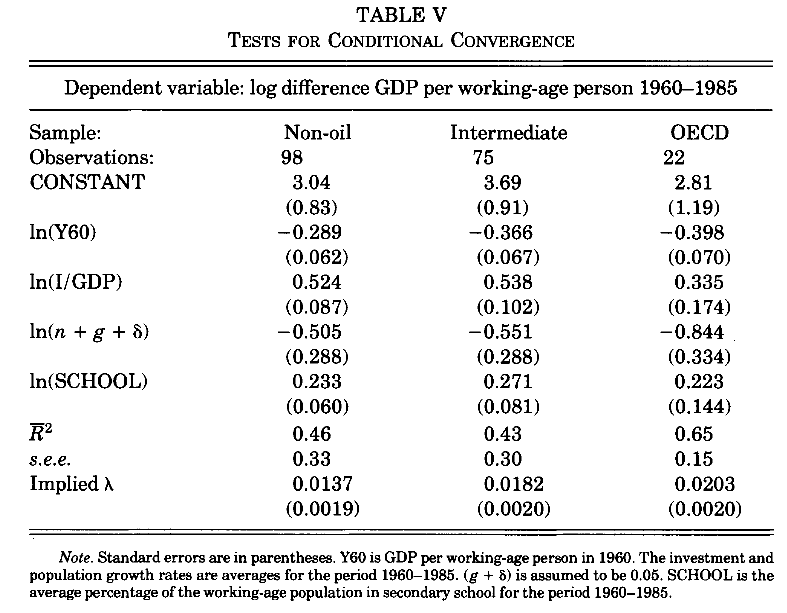
\includegraphics[scale=.40]{../img/mrw-table-5.png}
  \end{center}


\end{frame}


\end{document}


% Local Variables:
% ispell-check-comments: exclusive
% ispell-local-dictionary: "french"
% TeX-master: t
% End:
